\documentclass{llncs}

\usepackage[utf8]{inputenc}
\usepackage{tikz}

\usepackage{algorithm}
\usepackage{algorithmic}
\input{spanishAlgorithmic}

\title{Algoritmos Inmunes Artificiales en el UTRP}
\author{Cristopher Arenas\\\texttt{cristopher.arenas@alumnos.usm.cl}}
\institute{Departamento de Informática\\Universidad Técnica Federico Santa María}

\renewcommand{\tablename}{Tab. }

\begin{document}
\maketitle

\begin{abstract}
Los algoritmos inmunes artificiales (AIA) son estrategias de resolución de problemas evolutivos, lo que quiere decir que cambian con el tiempo y representan analogías de ciertos comportamientos biológicos. Estos algoritmos se puede utilizar en ciertos problemas, como por ejemplo el Urban Transit Routing Problem UTRP, en el cual se pretende encontrar rutas que satisfagan a operadores de los buses y a las personas que transportan. Por medio de un modelamiento, una representación del problema y la resolución por medio de un AIA se encontrará una solución que pueda satisfacer un conjunto de restricciones y trabajar con ciertos objetivos.
\end{abstract}

\section{Introducción}

Existen acercamientos que se encargan de resolver el Urban Transit Routing Problem (UTRP) \cite{metaheuristic2010}. Entre ellos se encuentran algoritmos evolutivos que emulan ciertos comportamientos de la naturaleza y los organismos de manera de encontrar soluciones a este tipo de problemas. \\

Dentro del grupo de los algorimos evolutivos, existen algunos que implementan ciertos comportamientos observados en los organismos de las personas. Los algoritmos inmunes artificiales representan una metáfora del sistema inmune donde se tiene un conjunto de anticuerpos que tienen la misión de encargarse de los virus y bacterias de enfermedades que atacan a un organismo. Los anticuerpos funcionan a través de procesos adaptativos, pues una vez que encuentran la mejor forma de curar una enfermedad se capacitan para futuras infecciones \cite{introduction} \cite{sia}. \\

En el presente documento se implementará un algoritmo evolutivo que se enfoca en simular el comportamiento del sistema inmune para resolver el UTRP. Posteriormete, se escogeran parámetros adecuados para el problema mediante un proceso de sintonización. Finalmente, se mostrarán algunos experimentos con instancias y las conclusiones del trabajo realizado.

\section{Estado del Arte}
El problema de enrutamiento de tr\'ansito urbano (UTRP por sus siglas en ingl\'es) involucra la ideaci\'on de rutas para el transporte p\'ublico.
Se trata de un problema NP-Duro altamente complejo, y resolverlo involucra invariablemente un ciclo de
generaci\'on y prueba de grupos de rutas candidatas. La mayor parte de literatura lo considera parte de un problema de escala mayor, el Urban Transit Network Design Problem (UTNDP por sus siglas),
el cual es dividido tanto en el UTRP como UTSP (Urban Transit Scheduling Problem), y tal como se puede diferir de sus nombres, el UTSP
tiene un enfoque de agendar los tiempos de llegada de los medios de transporte, mientras que el UTRP se enfoca en las rutas que estos
utilizan, ambos para mejorar el sistema de transporte urbano en las ciudades.\\
Los primeros acercamientos al UTRP lo tratan como un problema mono-objetivo. En~\cite{metaheuristic2010} se
comparan dos acercamientos de b\'usqueda local para resolver el problema. En este
caso se consideran dos objetivos: la distancia acumulada de todos los pasajeros
del bus y el n\'umero de trasbordos para la demanda completa. Se considera toda la demanda como satisfecha y el tiempo
promedio que cada usuario destina en viajar es
el menor posible. Adem\'as, se considera que cada ruta del conjunto est\'a libre de ciclos y retrocesos;
el conjunto de rutas est\'a conectado; hay exactamente $r$ rutas en el conjunto y el n\'umero de nodos en cada
ruta debe ser mayor a uno y no debe exceder el valor m\'aximo definido. \\
La funci\'on objetivo est\'a dada por la suma ponderada de ambos objetivos.
La inicializaci\'on se realiza de manera aleatoria respetando el largo establecido. Se
utiliza el movimiento \emph{Make-small-change}, que considera 3 posibilidades: Agregar un nodo en
la \'ultima posici\'on de la ruta, borrar el primer nodo de la ruta e invertir el orden de nodos en la ruta.
En~\cite{memetic2011} se propone un algoritmo mem\'etico cuyo objetivo es minimizar la suma del costo
para los usuarios y la demanda insatisfecha para la red de rutas. La inicializaci\'on se reliza
de manera aleatoria, se utiliza cruzamiento de rutas en un punto y mutaci\'on de una ruta por otra ruta factible. Para
la b\'usqueda local se seleccionan uno o dos cromosomas aletatoriamente, y se combinan de acuerdo a: (1) 
movimiento 2-opt, (2) intercambio de dos paraderos y (3) reubicaci\'on de una parada. Al final del proceso
se seleccionan los mejores $\mu$ cromosomas padre y $\lambda$ cromosomas hijo.
En~\cite{jiang2010improved} se utilizan colonias de hormigas para el UTRP. A diferencia de otros problemas resueltos con colonias de
hormigas, las hormigas no deben recorrer todos los nodos, sino que deben ir desde cierto nodo hasta otro.
Se toma como consideraci\'on que cada nodo podr\'a tener a lo m\'as 4 vecinos y las conexiones con estos ser\'an aquellas pertenceciente a
un conjunto de arcos permitidos. Si en alg\'un momento la ruta escogida por la hormiga no cumple
alguna de las restricciones (por ejemplo, ciclos en el recorrido), la hormiga se declara muerta y se castiga el
camino escogido.\\

Es posible encontrar acercamientos multi-objetivo para otros problemas similimares. Josefowiez, Semet y Talbi
en~\cite{vrprb} utilizan diversificaci\'on elitista y modelo de islas para el vehicle routing problem con
dos objetivos: minimizaci\'on del largo de las rutas y la diferencia entre el tama\~no de la ruta m\'as larga y la m\'as corta.
En este caso se utiliza ranking de dominancia para evaluar a los invididuos, donde los individuos no dominados de la poblaci\'on
forman el conjunto $E_1$ de ranking 1 y el resto de los individuos se agrupan en conjuntos $E_k$ donde cada elemento es dominado
por todos los elementos de los conjuntos anteriores.
En~\cite{ttvrp} se propone un MOEA h\'ibrido que incorpora b\'usqueda local y el concepto de optimalidad de Pareto para el
problema de encontrar una programaci\'on de rutas que cumpla con todas las entregas de una empresa de despacho, minimizando las distancias
recorridas y el n\'umero de camiones. Al igual que en el caso anterior se utiliza un ranking de fitness de Pareto para evaluar la calidad
de las soluciones. Zhang, Wang y Tang~\cite{events} investigan el problema de dise\~no de rutas para mega-eventos donde hay un gran
tr\'afico de transporte p\'ublico y se requieren rutas adicionales para el transporte de las personas que participan de un evento,
a su lugar de destino. En~\cite{events} se utiliza un algoritmo gen\'etico cuya funci\'on de evaluaci\'on es la distancia total del
conjunto de rutas. Adem\'as, se utilizan dos penalizaciones: la primera se aplica por cada nodo de destino que qued\'o fuera de ruta y
la segunda se aplica si la distancia total de una ruta supera la m\'axima distancia permitida.\\

Acercamientos multi-objetivos espec\'ificos para el UTRP se pueden encontrar en~\cite{zhang2010multi} donde se utiliza un algoritmo
evolutivo que usa el operador \emph{Make-small-change}. En este caso se utiliza el concepto de dominancia de Pareto para construir
el conjunto de soluciones. Este algoritmo entrega buen conjunto de rutas desde el punto de vista de los pasajeros y con mejores costos
para operadores en comparaci\'on a un algoritmo mono-objetivo similar con el que se compar\'o. Mumford en~\cite{NewHaEOps} utiliza exactamente
el mismo modelado, pero agrega un operador de cruzamiento al algoritmo evolutivo. El operador de cruzamiento selecciona intercaladamente
rutas de ambos padres de manera tal de tener una cantidad equitativa de rutas de cada padre en el hijo. En~\cite{GAUTRP}
se considera el mismo modelo y funci\'on objetivo que los anteriores, pero 
se realizan diferentes operaciones sobre un set de rutas para tratar de mejorar su calidad. Entre las modificaciones
se encuentran: una selecci\'on mediante ruleta de las rutas a modificar, una operaci\'on crossover entre dos rutas padres,
y la revisi\'on de factibilidad de los hijos, para finalmnente realizar una operaci\'on de mutaci\'on sobre dos rutas pertenecientes
al mismo set, intercambiando nodos aleatorios.\\

Para hacerse una idea de la complejidad real del problema es posible mencionar que el sistema de transportes de la ciudad de Santiago, Chile,
Transantiago cuenta con $372$ recorridos, y $11272$ paradas disponibles. Dichas paradas se distribuyen en siete unidades agrupadas por
zonas~\cite{datosGob}. Adem\'as, cuenta con 7 tipos de servicios entre los que se cuentan: servicios normales, cortos, expresos, variantes,
nocturnos, especiales e inyectados que operan en distintas condiciones horarias y de capacidad. Los estudios realizados en el caso
particular de Santiago coonsideran microsimulaciones de focos de congesti\'on considerando
diferentes escenarios de aumento de la capacidad vial, reversibilidad de las pistas y simulaci\'on de incidentes~\cite{alarcon2010}, 
mientras que en~\cite{cortes2009} se presenta un metodo de resoluci\'on para el problema de asignaci\'on de horarios, rutas y asignaci\'on
de choferes para una de las siete empresas del Transantiago (STP Santiago) que cuenta con aproximadamente 300 buses.
El autor aborda el problema mediante MIP (Programaci\'on Entera Mixta).

\section{Descripción del problema}

El problema considera inicialmente que se cuenta con algunas variables, tales como un grafo $G$; el cual representa una red de paraderos, lo que se puede entender, por ejemplo, como la estructura que se tiene en una ciudad. Cada vértice corresponde a un paradero, mientras que los arcos corresponden a las conexiones o caminos existentes entre dichos paraderos. Se considera que el grafo es no dirigido, lo que quiere decir que un arco entre dos vértices indica que hay una conexión en ambos sentidos entre los arcos que conecta. Las posiciones de cada vértice también son conocidas. Además, este grafo posee matrices simétricas, que poseen valores de tiempo de viaje entre paradas, demandas asociadas para cada vértice.

Como restricciones del problema se puede considerar lo siguiente \cite{NewHaEOps}:
\begin{itemize}
\item Cada ruta del conjunto de rutas está libre de ciclos y retrocesos.
\item El conjunto de rutas está conectado.
\item Hay exactamente $r$ rutas en el conjunto de rutas.
\item El número de nodos en cada ruta debe ser mayor a uno y no debe exceder el valor máximo definido.
\end{itemize} 

Con esto se asume que se sabe cuantas rutas tendrá el conjunto de rutas resultante, además de que tendrán un rango paraderos permitidos, los cuales están acotados por un mínimo y un máximo.

El UTRP consiste en satisfacer tanto a operadores de buses, como a los pasajeros que los utilizan. Es por esto que se tienen las siguientes funciones objetivo (\ref{eq:fo1}) (\ref{eq:fo2}) \cite{NewHaEOps}.

\begin{equation}
\label{eq:fo1}
min\mbox{ }\frac{\sum^n_{i,j=1}d_{ij}\alpha_{ij}(R)}{\sum_{i,j=1^n}d_{ij}}
\end{equation} 

\begin{equation}
\label{eq:fo2}
min\mbox{ }\sum^r_{a=1}\sum_{(i,j) \in r} t_{i,j} (a)
\end{equation} 

La función objetivo (\ref{eq:fo1}) considera los costos del operador. $d_{ij}$ representa la demanda  entre las paradas $i$ y $j$ y $\alpha_{ij}$ corresponde al camino más corto entre las dos paradas. Por otra parte, la función objetivo (\ref{eq:fo2}) corresponde a los costos del pasajero. $t_{ij}$ corresponde al tiempo de viaje entre las paradas $i$ y $j$. Los costos que se pretende satisfacer es la demanda, por parte de los operadores y los tiempos de viaje por parte de los pasajeros.

\section{Representación}

Dentro del contexto del UTRP, se pretende determinar un conjunto de rutas a partir de distintos paraderos de buses preestablecidos, los cuales deben presentar un beneficio para los pasajeros y para el operador del bus.\\

Para las paradas se utiliza un grafo no dirigido, cuyos vértices corresponden a las paradas y los arcos a un camino entre las paradas. Un ejemplo de esta representación es la red de Mandl, la cual puede apreciarse en la Figura \ref{fig:mandl}.

\begin{figure}[!htb]
\begin{center}
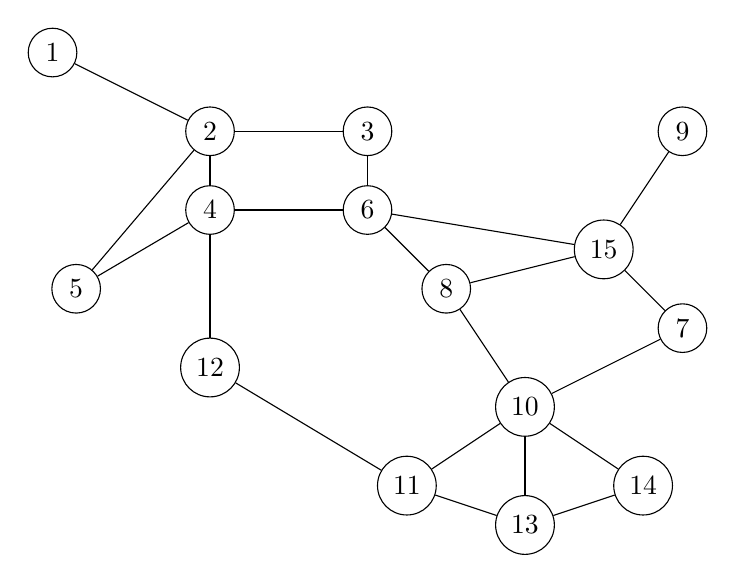
\begin{tikzpicture}
\node[draw,circle](1) at (0,0) { 1};
\node[draw,circle](2) at (2,-1) { 2};
\node[draw,circle](3) at (4,-1) { 3};
\node[draw,circle](4) at (2,-2) { 4};
\node[draw,circle](5) at (0.3,-3) { 5};
\node[draw,circle](6) at (4,-2) { 6};
\node[draw,circle](7) at (8,-3.5) { 7};
\node[draw,circle](8) at (5,-3) { 8};
\node[draw,circle](9) at (8,-1) { 9};
\node[draw,circle](10) at (6,-4.5) {10};
\node[draw,circle](11) at (4.5,-5.5) {11};
\node[draw,circle](12) at (2,-4) {12};
\node[draw,circle](13) at (6,-6) {13};
\node[draw,circle](14) at (7.5,-5.5) {14};
\node[draw,circle](15) at (7,-2.5) {15};

\draw (1) -- (2);
\draw (2) -- (3);
\draw (2) -- (4);
\draw (2) -- (5);
\draw (3) -- (6);
\draw (4) -- (5);
\draw (4) -- (6);
\draw (4) -- (12);
\draw (6) -- (8);
\draw (6) -- (15);
\draw (7) -- (15);
\draw (7) -- (10);
\draw (8) -- (10);
\draw (8) -- (15);
\draw (9) -- (15);
\draw (10) -- (11);
\draw (10) -- (13);
\draw (10) -- (14);
\draw (11) -- (12);
\draw (11) -- (13);
\draw (13) -- (14);
\end{tikzpicture}
\caption{Red de Mandl}
\label{fig:mandl}
\end{center}
\end{figure}

La representación escogida para manejar el UTRP es mediante un arreglo bi-dimensional que representa un conjunto de rutas. Cada fila será una ruta, la cual contiene un identificador asociado al número de ruta y posteriormente identificadores para las paraderos de buses. Estos paraderos se encuentran representados por una matriz de demandas, una matriz de tiempos de viaje y por un sistema de coordenadas (este último para modelar la posición de cada paradero).

En la Figura \ref{fig:repr1} se muestra un ejemplo de una representación de rutas el cual se pudo obtener a partir de la literatura existente sobre el UTRP \cite{metaheuristic2010}.

\begin{figure}[!htb]
\begin{center}
\begin{tabular}{|p{0.8cm}|p{0.8cm}|p{0.8cm}|p{0.8cm}|p{0.8cm}|}
\hline
R1 & 0 & 1 & 4 & 7\\
\hline
R2 & 0 & 3 & 6 & $*$\\
\hline
R3 & 1 & 2 & 5 & $*$\\
\hline
\end{tabular}
\caption{Representación para las rutas.}
\label{fig:repr1}
\end{center}
\end{figure}

Las matrices de tiempos de viaje y de demandas se representan mediante arreglos bidimensionales, donde la fila $i$ y columna $j$ aporta información entre el paradero $i$ y el paradero $j$.\\

Las soluciones para el algoritmo inmune artificial propuesto están dadas por un conjunto de rutas que siguen la estructura de la Figura \ref{fig:repr1}.

\section{Estructura del algoritmo}

El Algoritmo \ref{alg:aia} muestra a grandes rasgos el pseudocódigo del algorimto artificial inmune implementado. Un anticuerpo se entiende dentro del contexto de los algoritmos inmunes artificiales como una solución candidata.

\begin{algorithm}
\caption{Algoritmo Inmune Artificial}\label{alg:aia}
\begin{algorithmic}[1]
\STATE Inicializar población de anticuerpos aleatoriamente con sets de rutas factibles
\STATE $g=0$
\WHILE{\texttt{GENERACIONES}$>g$}
	\STATE Eliminar de la población anticuerpos dominados en cada set
	\STATE Calcular afinidad de cada miembro de la población
	\STATE Clonar $a$ de los mejores anticuerpos hsata llegar a un tamaño \texttt{CLON\_SIZE}
	\FOR{\textbf{cada} Clon}
		\STATE Mutar Clon
	\ENDFOR
	\STATE Guardar $b$ mejores anticuerpos	
	\STATE Eliminar exceso de anticuerpos
	\STATE Reemplazar peores anticuerpos con anticuerpos generados aleatoriamente
	\STATE $g=g+1$
\ENDWHILE
\end{algorithmic}
\end{algorithm}

En el pseudocódigo se pueden disinguir ciertas etapas que serán detalladas a continuación.

\section{Inicialización}

La inicialización del conjunto de soluciones inicial es determinado de manera aleatoria. De tal forma de tener contar con distintos lugares del espacio de búsqueda. Cada solución del conjunto contiene un conjunto de rutas, escogido de la siguiente manera: aleatoriamente se escoge un largo de ruta, el cual está comprendido entre el mínimo y máximo establecido. Se escoge aleatoriemente un punto de partida y se genera un camino mediante las conexiones con paradas vecinas hasta completar el largo. Se realiza este procedimiento hasta tener un conjunto de rutas que posea todos los paraderos disponibles o hasta que se agote un número de intentos, lo que puede ocurrir cuando el número de paraderos es muy grande en comparación con la cantidad de paraderos que serán destinados a una ruta o si el número de rutas a generar es muy pequeño. Las instancias con las que se trabajará siempre tratarán de incluír a todos los paraderos.\\

Se genera una población de soluciones de manera de tener varias soluciones candidatas. Este conjunto de soluciones inciales es un conjunto de soluciones factible, lo que quiere decir que las rutas generadas son conexas y además no presentan ciclos ni backtrackings. El algoritmo trabaja con soluciones factibles y al generar nuevas soluciones se comprueban las condiciones necesarias para que también sean factibles. 

\section{Proceso de transformación}

\subsection{Selección de soluciones}

El primer paso en el proceso de transformación del algoritmo consiste en realizar una selección clonal. Esto es, seleccionar a los mejores anticuerpos en base a una función de aptitud (\ref{eq:faptitud}). 

\begin{equation}
\label{eq:faptitud}
f_{aptitud}=\alpha \cdot FO_1 + \beta \cdot FO_2
\end{equation}

Donde $FO_1$ y $FO_2$ corresponden a las funciones objetivo dadas por las ecuaciones (\ref{eq:fo1}) y (\ref{eq:fo2}), respectivamente. Un porcentaje de estas soluciones son escogidas de acuerdo al resultado de $f_{aptitud}$ para pasar a la siguiente etapa del algoritmo.

\subsection{Operadores de transformación}

Los mejores anticuerpos son clonados hasta llegar a una cierta población. Esto consiste básicamente en generar muchas copias de los mejores anticuerpos. El operador de selección toma un anticuerpo y genera uno igual. La manera de decidir cual de los mejores anticuerpos se clona se realiza de manera aleatoria. De esta forma cada uno de los anticuerpos tiene la misma probabilidad de ser clonado.\\

Posteriormente, se utiliza un operador de mutación, el cual consiste en introducir pequeños cambios al conjunto de rutas para producir cambios en sus funciones objetivo, y por ende en la función de aptitud. La mutación consiste en seleccionar aleatoriamente una ruta de una solucion e introducir un nuevo vertice en ella, siempre y cuando no exceda el límite superior.


\subsection{Selección de soluciones para conformar nueva población}

Luego, se aplica una reducción de la población de los clones, dejando los más aptos (con una mejor función de aptitud). Se procede a reemplazar a los peores anticuerpos con anticuerpos generados aleatoriamente, siguiendo las mismas restricciones de la generación inicial al generar soluciones candidatas factibles. 

\section{Parámetros del algoritmo}

El algoritmo considera los siguientes parámetros:

\begin{itemize}
\item \texttt{POP\_SIZE}: Representa el tamaño de la población en cada generación. Una generación está compuesta por un conjunto de soluciones candidatas. Posee valores de 0 a infinito.
\item \texttt{ALPHA} y \texttt{BETA}: representan variables de peso para ponderar las dos funciones objetivo y determinar una aptitud para la solución candidata. Posee valores entre cero y uno. La suma de ambas debe ser uno.
\item \texttt{CLON\_SIZE}: cantidad de clones que se generarán a partir de las mejores soluciones candidatas.  Posee valores de 0 a infinito.
\item \texttt{AFINIDAD}: Porcentaje de mejores soluciones seleccionadas para mutarse. Posee valores entre 0 y 1.
\item \texttt{GENERACIONES}: Cantidad de generaciones que se producirán hasta la finalización del algoritmo. Posee valores de 0 a infinito.
\item \texttt{CLONES}: porcentaje de clones que sobrevivirá después de realizar el operador de mutación. Posee valores entre 0 y 1.
\item \texttt{REEMPLAZO}: porcentaje de anticuerpos que serán reemplazados por nuevos anticuerpos aleatorios. Posee valores entre 0 y 1.
\end{itemize}

\section{Sintonización de Parámetros}

Para la sintonización de parámetros se escogieron 4 de los parámetros y el resto quedó con un valor fijo. Entre los parámetros con valor fijo se utilizaron los valores de la Tabla \ref{tab:paramfijos}. La instancia utilizada fue la de \texttt{Mandl 6:2:8}, cuyo grafo está representado en la Figura \ref{fig:mandl}. Se buscan 6 rutas con longitudes que varían en el rango de 2 a 8 paradas.

\begin{table}[!htb]
\begin{center}
\begin{tabular}{|c|c|}
\hline
\texttt{ALPHA} & 1.0\\ \hline
\texttt{BETA} & 1.0\\ \hline
\texttt{AFINIDAD} & 1\\ \hline
\texttt{REEMPLAZO} & 0.01\\ \hline
\end{tabular}
\label{tab:paramfijos}
\caption{Parámetros seteados en un valor fijo para Mandl.}
\end{center}
\end{table}

Los parámetros \texttt{POP\_SIZE}, \texttt{CLON\_SIZE}, \texttt{GENERACIONES} y \texttt{CLONES} fueron puestos a prueba al utilizar ParamILS, un sintonizador de parámetros que utiliza un intérprete del código y ejecuta el algoritmo utilizando un rango de valores para los 4 parámetros escogidos.

\begin{figure}[!htb]
\begin{verbatim}
ps {20, 40, 100, 160, 200}[100]
cs {5, 15, 25}[15]
it {10, 30, 50, 70, 100}[30]
pc {10, 30, 50}[10]
\end{verbatim}
\caption{Valores utilizados en los parámetros sintonizados en Mandl.}
\label{fig:paramsintonizados}
\end{figure}

En la Figura \ref{fig:paramsintonizados} \texttt{ps}, \texttt{cs}, \texttt{it} y \texttt{pc} corresponden a \texttt{POP\_SIZE}, \texttt{CLON\_SIZE}, \texttt{GENERACIONES} y \texttt{CLONES} respectivamente.

\newpage

Al ejecutar ParamILS se obtuvo la siguiente salida:

\begin{small}
\begin{verbatim}
Final best parameter configuration: cs=5, it=100, pc=10, ps=200
==================================================================
Active parameters: cs=5, it=100, pc=10, ps=200
==================================================================
Training quality of this final best found parameter configuration: 
-704.619631901841, based on 163 runs with cutoff 1000000000.0
Test quality of this final best found parameter configuration: 
-703.96, based on 50 independent runs with cutoff 1000000000.0
\end{verbatim}
\end{small}

Para este valores de parámetros se obtuvo un valor máximo de hipervolumen igual a 703.96.

\section{Experimentos}

El experimento con los valores de parámetros fijados según la Tabla \ref{tab:paramfijos} y los obtenidos mediante ParamILS, según lo mostroado a continuación:

\begin{table}[!htb]
\begin{center}
\begin{tabular}{|c|c|}
\hline
POP SIZE & 200\\ \hline
ALPHA & 1.0\\ \hline
BETA & 1.0\\ \hline
CLON SIZE & 5\\ \hline
AFINIDAD & 1\\ \hline
GENERACIONES & 100\\ \hline
CLONES & 0.1\\ \hline
REEMPLAZO & 0.01\\ \hline
\end{tabular}
\caption{Valores utilizados para el experimento con la instancia de Mandl.}
\end{center}
\end{table}

Notar que el porcentaje de clones fue manejado en ParamILS con valores entre 0 y 100 y pasado posteriormente a valores entre 0 y 1.

\begin{figure}[!htb]
\begin{center}
\includegraphics[scale=0.7]{pareto_mandl.png}
\caption{Frente de Pareto de la instancia de Mandl.}
\label{fig:pareto_mandl}
\end{center}
\end{figure}

\begin{table}[!htb]
\begin{center}
\begin{tabular}{|l|c|}
\hline
Hipervolumen & 698.452\\ \hline
Tiempo de ejecución & 23 segundos\\ \hline
\end{tabular}
\caption{Hipervolumen y tiempo de ejecución.}
\label{tab:mandldata}
\end{center}
\end{table}

Además, los mejores valores para las funciones objetivo corresponden a:
\begin{itemize}
\item Mejor FO1: 11.5087
\item Mejor FO2: 76
\end{itemize}

\newpage
El conjunto de rutas que presenta el menor valor para la función de aptitud se muestra a continuación:
\begin{verbatim}
6-3
9-15-6-8
3-2-4-12
8-6-3
8-15-7-10-14-13-11
1-2-5
\end{verbatim}

Se puede concluir que estos resultados no reflejan exactamente a lo obtenido mediante la sintonización de parámetros porque esto corresponde solo a una ejecución del algoritmo. Por otra parte, ParamILS realiza una cantidad considerable de experimentos probando con distintos valores y logra encontrar el mejor valor de hipervolumen. En este caso el valor es cercano al mejor valor obtenido, sin embargo si se realizara otro experimento podría originar un valor más cercano o más lejano.

\section{Conclusiones}

Los algoritmos inmunes artificiales utilizan analogías de los organismos vivos. Cuando un virus ataca al organismo los anticuerpos son capaces de interactuar con este y los más capaces son duplicados para atacar y eliminar a una enfermedad que cause. Luego se guarda en memoria una cantidad menor de este anticuerpo para que esté preparado a nuevas infecciones del mismo virus o uno similar. Esta idea es la que permite encontrar soluciones mediante la clonación y mutación de los mejores individuos. El proceso de búsqueda de soluciones es un proceso adaptativo, lo que quiere decir que los anticuerpos se capacitan para enfrentarse a infecciones futuras. \\

Mediante esta implementación, la cual está compuesta por variables, restricciones, funciones objetivo, función de aptitud, operadores de selección y transformación para una población de anticuerpos se pudo encontrar un conjunto de soluciones no dominadas según Pareto, obteniendo mejores soluciones en tiempos relativamente cortos. \\

El proceso de sintonización de parámetros fue útil para poder encontrar valores para parámetros y obtener un mejor resultado, el cual está reflejado en un mayor valor de hipervolumen.\\


\section{Bibliograf\'ia}
\bibliographystyle{plain}
\bibliography{utrp}

\end{document}
